\documentclass{article}
\usepackage[utf8]{inputenc}

\title{Lecture 9: regression  }
\author{wbg231 }
\date{November 2022}
\usepackage{tikz,graphicx,amsmath,amsfonts,amscd,amssymb,bm,cite,epsfig,epsf,url}
\begin{document}

\maketitle

\section{introduction}
\subsection{history}
\begin{itemize}
%\item 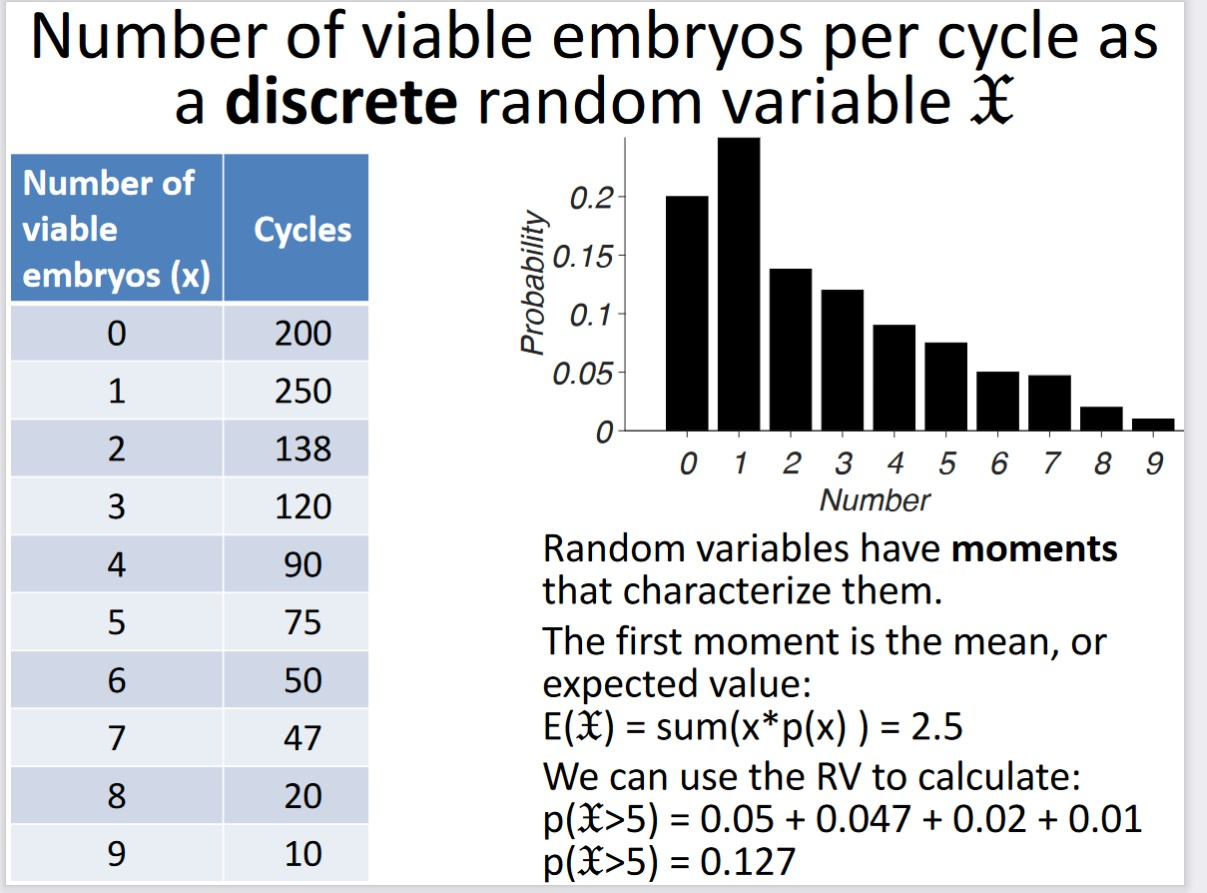
\includegraphics[width=7.5cm]{Final_Review/Lecture_2/lecture_1example.jpg}
\item making predictions has been a practice in every cloture ever
\item there is always someone who's job it is to make predictions about the future 
\item tea leaves, starts etc 
\subsection{data based predictions}
\item we want to predict some future outcome (y) based on the current known state (the predictor) 
\item the current state is a matrix 
\item we want to predict some outcome which will be a vector 
\item the most common prediction tool is regression 
\subsection{the rule of three}
\item let a,b,c be constants and x an unknown 
\item $\frac{a}{b}=\frac{c}{x}$ we can solve for x as $x=\frac{cb}{a}$
\item as people were digging deeper into the earth in England during the industrial revolution 
\item suppose we have we want to know the high of dins 2 and we know the hie hgt of dinosaur 1 as well as the thigh bone length of dinosaur 1 and 2 this can be expressed as $\frac{t_1}{h_1}=\frac{t_2}{x}$ where x is the height of the second animal 
\item we can literally solve for the height of the second animal, but that may not be a good idea because we are assuming linearity
\item also in the real world there is noise 
\itme it was shown by Glutton, that the rule of three over shoots the actual prediction 
\section{OLS regression}
\subsection{regression introduction}
\item the rule of three overshoots even linear relationships due to noise
\item his question is can we determine the height of children based on the height of their parents 
\item he found there was a statistical relationship, but the relationship is not perfect, the rule of three will systematically overshoot
\item this is where the term regression comes form, the data is regressing to the mean, if you are very tall you children are also likely to be tall, but not very tall. 
\item why is this? it is because height has nature nurture and other random factors that are involved, and can not be fully captured by genetics. 
\item so the whole method was named after this 
\subsection{linear regression analysis }
\item the predictor should be on the x, the outcome should be on the y, this was not the case in the earliest example
\item this plays a central role in many fields where we have a lot of data, but it is hard to do experiments 
\item in general we are looking for the unit effect of x on y, ie how much does y change in reasons to a one unit change on x 

\subsection{regression is not causation}
\item do identify causality you need an experiment regression is correlational. 
\item in simple linear regression it is looking for causation, but unless there is an experiment there could be confounders. for instance eating hot dogs could be effected by something else c that also effects y 
\subsection{linear regression }
\item linear regression is the relationship between the predictor and the outcome that can be accounted for by fitting a line 
\item if things are totally linear and there is no error then we can just draw a straight line 
\item in any other cases where will be scatter. 
\subsection{what is the best line for our data}
\item residuals is the distance between the real points and our line 
\item our goal in linear regression is minimize the sum of the squared residuals 
\item residuals are squared to prevent overshooting and undershooting from canceling out. 
\item this model assumes that over predicting and under predicting are equally as bad 
\subsection{terminology}

\item 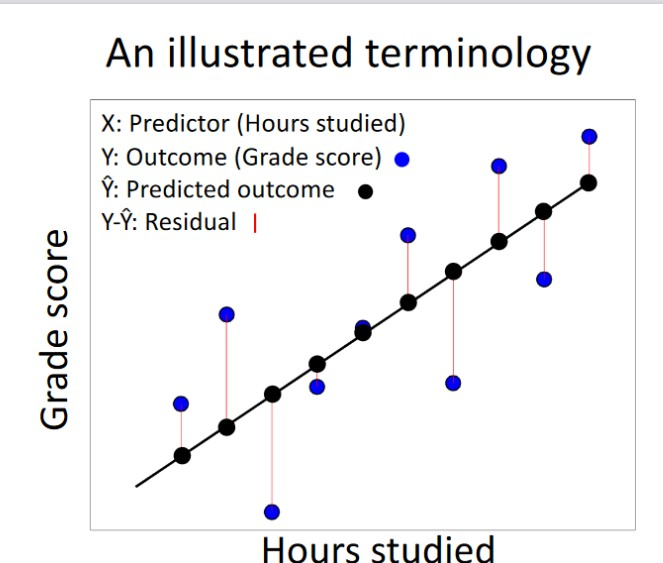
\includegraphics[width=7.5cm]{Final_Review/lecture_9/reg terminology .jpg}
\item X is predictor 
\item y is outcome 
\item $\hat{y}$ is our predicted outcome 
\item $y-\hat{y}$ are our residuals 
\item the goal of linear regression is $min f(x)=\Sigma(\text{risidual})^2\\=\Sigma(Y-\hat{y})^2=\Sigma(Y-\beta X)^2 $wrt $\beta \in \mathbb{R}$  
\item that is to find a single scalar beta that shrinks or stretches the x to approximate y as well as possible 
\item sum of squared residuals is a convex function, so we can find a good global minimum easily.it is also nice and differentiable so it is just a nice ez function to work with 
\item OLS has a global min and is differentiable everywhere 
\subsection{Linear algebra approach}
\item we solve for our $\beta_{ols}=\frac{<x,y>}{<x,x>}$ super easily using vector projections (did this in more detail in lecture 8)
\item we are using vector projection to make the prediction 
\item it is just the question how how to project our data (x) onto a single dimension y using vector projections 
\item dot products are very quick so this has low time complexity.
\item we could pick different distance metrics depending on our error function but in this case we are happy with just using the sum of squared residuals
\subsection{using regression to predict}
\item it f we have no information the ols can be minimized by always guessing the mean of y.  
\item however, if one knows the value fo the predictor value x and the correlation between x and y we can improve upon guessing the mean with regression 
\item regression critically relies on co relation 
\subsection{Regression to the mean line }
\item 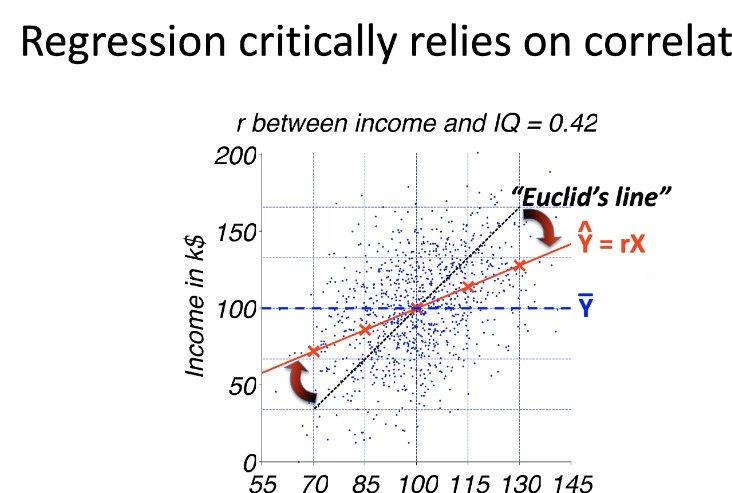
\includegraphics[width=7.5cm]{Final_Review/lecture_9/regresson_to_man_effect.jpg}
\item iq regressed on income
\itme the correlation between iq and income is .42
\item can we do better than just guessing the mean? yes because there is a relationship (the blue line)
\item suppose we add grid lines connecting the standard deviation in x and y, is a good line just connecting the vertices of the standard deviations good? no, because it is too steep, it does not move with the mean, this is predicting a perfect correlation, which is not the case here.  (this is the black line called euclid;s line)
\item the best fit line is that for every one unit of standard deviation in x, we move over by .42 (the correlation between x and y) units of y this is the red line 
\item the regression to the mean effect is the angle between Euclid's line and the OLS line 
\item if the correlation is very strong the regression to the mean effect is small 
\item if the correlation is week the regression to the mean effect is large 
\item if there is no correlation then the mean is the best guess 
\subsection{problem with regression for prediction}
\item you work as a data scientist for the government  want to make nutritional recommendations 
\item you are told that there is a Strong correlation between the intake of red meat and heart disease. should you tell people to stop eating red meat? no correlation is not causation. but then you are told that a regression analysis was run and red meat is predictive of heart disease . don't but this regression is just causation 
\item OLS on its own does not control for confounders, so it does not mean causation unless we are controlling for other things 
\item to make a causal statement we need to control for confounds
\item new York time want to live longer go to the opera,but that is related to wealth which is related to living longer
\section{General linear models}
\subsection{The case for multiple regression}
\item you can not compare apples and oranges because they are different
\item multiple regression allows us to compare apples and oranges explicitly by acknowledging there known differences
\item there is a positive statistical relationship between smoking and lung cancer controlling for wealth and age
\item age and wealth are confounds for this relationship
\item fisher maintained that smoking does not cause cancer. 
\item we proved it does cause cancer because of analog experiences 
\subsection{example}
\item x number of students y learning outcomes 
\item is x related to y
\item we can not really run an experiment on this because people will not comply 
\item so instead we instead look at the model 
\item suppose we start with a simple linear regression and find there is no relationship
\begin{itemize}
\item but we did not control for any confounds, like teach experience, wealth if it is a good school overall etc. 
\item so say our sample space for the simple linear model looks like this 
\item 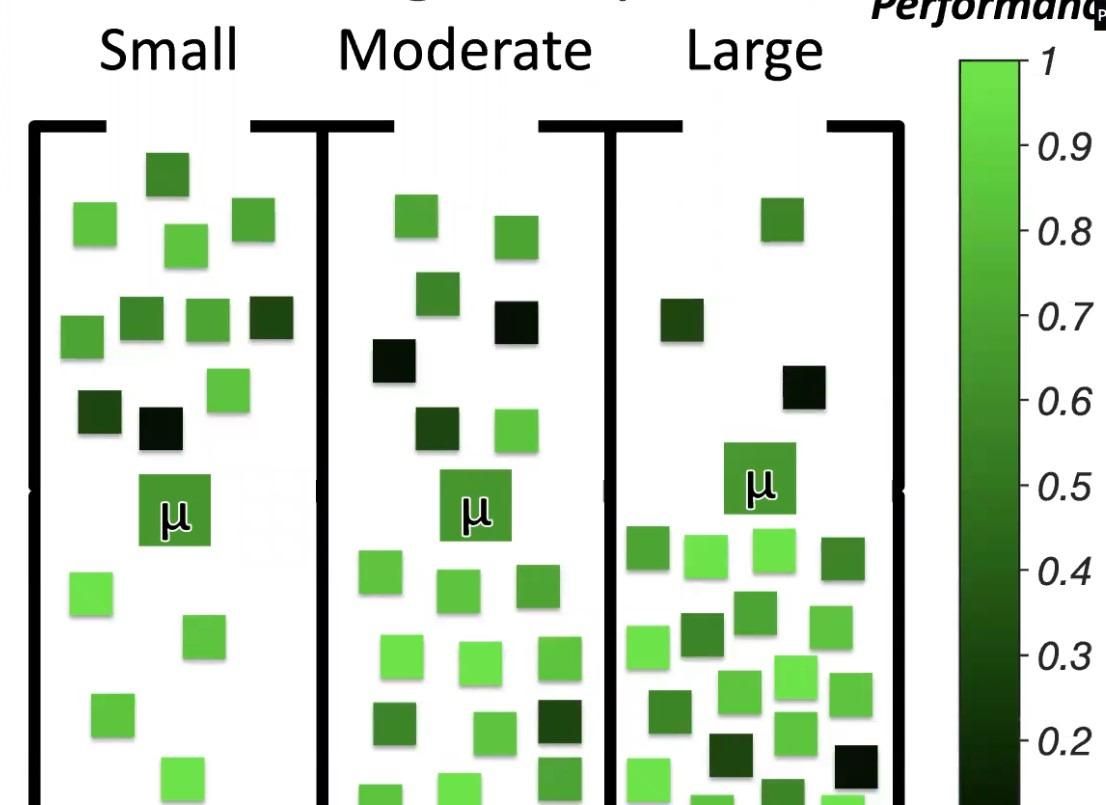
\includegraphics[width=5cm]{Final_Review/lecture_9/sample_space_1.jpg}
\end{itemize}
\item so we use multiple regression to control for some of this and some divide on behavioral issues so our sample space looks like this\item  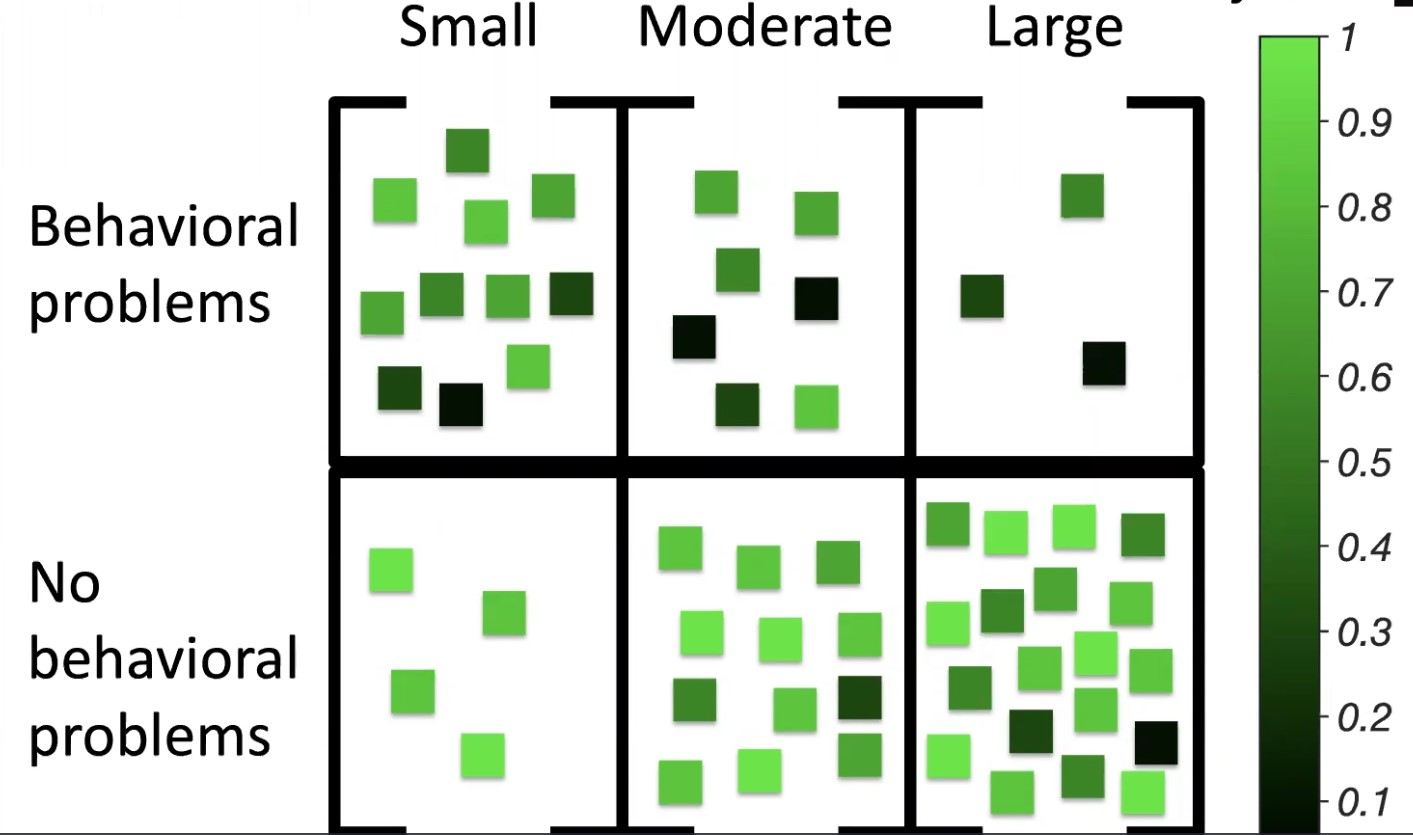
\includegraphics[width=5cm]{Final_Review/lecture_9/sample_space_2.jpg}
\item we see that as class size goes up, student learning outcomes go down 
\item but we did not control for many other confounds 
\item we can keep controlling for more confounds and subdividing our space
\subsection{multiple regression take away}
\item the gold standard is experiments 
\item but multiple regression models are the next best thing, they implement all things equal (ceteris paribus) 
\item suppose we have 1 predictor classroom size small versus large then we subdivide our space in 2 pieces
\item then we add behavioral problems as a binary so we have subdivided out space into 4 areas
\item adding n binary variables subdivides our space into $2^n$ cells
\item due to the curse of dimensionality as our cell number goes up there are less data in each cell 
\item we need to find a unique $\beta$ for each dimension that we add
\item so we want a trade off between a simple and a good model 
\subsection{General linear model}
\item $\beta\in \mathbb{R}^m$ is our parameters coefficients scales or weights
\item X is our matrix of independent variables $X\in \mathbb{R}^{nXm}$
\item y is our outcome $y\in\mathbb{R}^n$
\item simple linear regression can be expressed as $y=\beta_0+\beta_1X_1+\epsilon$ (this is a line in $\mathbb{R}^m$
\item we can generalize this as $y=\beta_0+\beta X +\epsilon$ this is a hyper plain in $\mathbb{R}^m$
\item the curse of dimensional means data requirements go up as dimensions go up 
\subsection{do people still use GLM}
\item deep learning models often predict better, but GLM models often lead to simple models
\itme the parameters in our GLM model are interpretative, in a way that they are not in deep leaning models
\item if $|\beta_i|$ tells us how much factor i contributes to y 
\item this does not lead to the best prediction  but it is understandable
\subsection{why OLS is still used}
\item simple easy to use 
\item coefficients are understandable 
\item it is fast
\item there is a global min
\subsection{ multiple linear regressions with linear algebra}
\item we still know that e=y-x$\Beta$
\item and $x\perp e$
\item thus we know hat $0=<X,e>=X^t(y-X\beta)\Rightarrow -X^TX\beta=-X^ty$
\item $\beta= (X^tX)^{-1}x^ty$ we know that $(x^tX)$ is invertible 
\item it geometrically looks the same we are kind of minimizing the sum of residuals in all dimensions 
\section{model assessment }
\item 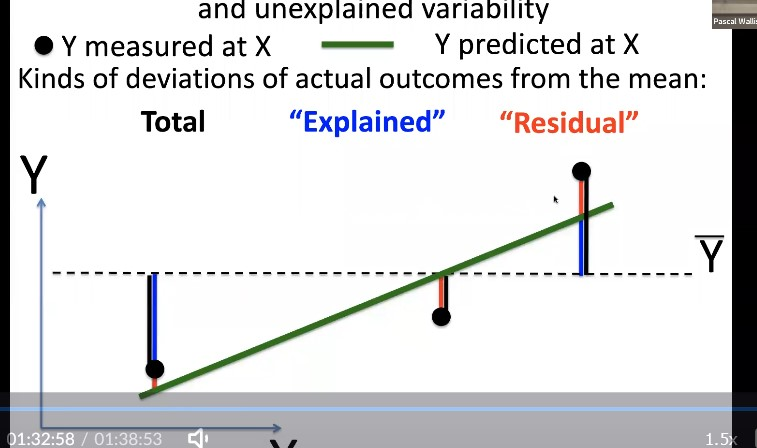
\includegraphics[width= 5cm]{Final_Review/lecture_9/R^2 i guess.jpg}
\item the variability in y can be broken down into two pieces, the part explained by the model and the part that we can not account for with the linear model 
\item total viability is the black distance from the mean of the model to the points 
\item the explained variability is the distance from the our line to the the mean 
\item then the residual is the distance between the actual outcome and the prediction
\item multiple regression is about maximising the explained variance and minimizing the residuals 
\subsection{Model Assessment terminology}
\item outcome y 
\item mean of the predictor $\Bar{y}$
\item predictions $\hat{y}=\beta X$
\item the residuals $(\Hat{Y}-Y)$
\item the sum of squared explained is thus $SS_{e}=\Sigma(\Hat{y}-\Bar{y})^2$ this is the total varinace that is explained by our model
\item the sum of squared residuals is $SS_{r}=\Sigma(\Hat{y}-y)^$
\item The coefficient of determination is thus $COD=\frac{SS_{E}}{SS_{E}+SS_{R}}$ this is the proportion of the error that is eplxained by our model 
\subsection{Metrics }
\item R (the correlation) is the correlation between our prediction $\hat{y}$ and y 
\item $R^2$ is the coefficient of determination, $COD=\frac{SS_{E}}{SS_{E}+SS_{R}}=R^2$
\item i think the COD is $R^2$ because we are squaring the sum of our sum of squared errors


\end{itemize}


\end{document}
